

\section{Experiment Details and Additional Results}\label{app:gnn_ablations}

\begin{table}
    % \vspace{-40pt}
    \caption{Entity classification results (AUROC mean$_{\pm \text{std}}$ over $5$ runs, higher is better) on \relbench. Best values are in bold along with those not statistically different from it.
    % \jure{What are these subscripts. Can you explain in the caption. Why are sometimes both methods bolded.} \jure{Remove subscripts, bold the max value; create another table in appendix with standard errors.}
    }
    \centering
    % \setlength{\tabcolsep}{3pt}
    % \scriptsize
    \tiny
    \CatchFileDef{\tabledata}{tables/app_node_classification.tex}{}
    \begin{tabular}{lllrr}
    \toprule
    \textbf{Dataset} & \textbf{Task} & \textbf{Split} & \textbf{LightGBM} & \textbf{RDL} \\
    \midrule
    \tabledata
    \bottomrule
    \end{tabular}
    \label{tab:app_classif}
\end{table}

\begin{table}
\caption{Entity regression results (MAE mean$_{\pm \text{std}}$ over $5$ runs, lower is better) on \relbench. Best values are in bold along with those not statistically different from it.
% \jure{same question here}
}
\centering
\setlength{\tabcolsep}{4pt}
% \scriptsize
\tiny
\CatchFileDef{\tabledata}{tables/app_node_regression.tex}{}
\begin{tabular}{lllrrrrrrr}
\toprule
\textbf{Dataset} & \textbf{Task} & \textbf{Split} & \makecell{\textbf{Global}\\\textbf{Zero}} & \makecell{\textbf{Global}\\\textbf{Mean}} & \makecell{\textbf{Global}\\\textbf{Median}} & \makecell{\textbf{Entity}\\\textbf{Mean}} & \makecell{\textbf{Entity}\\\textbf{Median}} &
\textbf{LightGBM} &
\textbf{RDL}\\
\midrule
\tabledata
\bottomrule
\end{tabular}
\label{tab:app_regression}
\end{table}

\begin{table}
\caption{Link prediction results (MAP mean$_{\pm \text{std}}$ over $5$ runs, higher is better) on \relbench. Best values are in bold along with those not statistically different from it.
% \jure{again same}
% \jure{to all tables, can be get avg. relative improvement/difference between RDL and DT?}
}
\centering
% \setlength{\tabcolsep}{4pt}
% \scriptsize
\tiny
\CatchFileDef{\tabledata}{tables/app_link_prediction.tex}{}
\begin{tabular}{lllrrrrr}
\toprule
\textbf{Dataset} & \textbf{Task} & \textbf{Split} &
\makecell{\textbf{Global}\\\textbf{Popularity}} & \makecell{\textbf{Past}\\\textbf{Visit}} &
\textbf{LightGBM} &
\makecell{\textbf{RDL}\\\textbf{(GraphSAGE)}} & \makecell{\textbf{RDL}\\\textbf{(ID-GNN)}} \\
\midrule
\tabledata
\bottomrule
\end{tabular}
\label{tab:app_link}
\end{table}

\subsection{Detailed Results}

Tables \ref{tab:app_classif}, \ref{tab:app_regression} and \ref{tab:app_link} show mean and standard deviations over $5$ runs for the entity classification, entity regression and link prediction results respectively.

\subsection{Hyperparameter Choices}

All our RDL experiments were run based on a single set of default task-specific hyperparameters, \emph{i.e.} we did not perform exhaustive hyperparamter tuning, \emph{cf.}~Table~\ref{tab:hparams}.
This verifies the stability and robustness of RDL solutions, even against expert data scientist baselines. Specifically, all task types use a shared GNN configuration (a two-layer GNN with a hidden feature size of $128$ and ``sum'' aggregation) and sample subgraphs identically (disjoint subgraphs of $512$ seed entities with a maximum of $128$ neighbors for each foreign key).
Across task types, we only vary the learning rate and the maximum number of epochs to train for.


\begin{table}[t]
  \centering
  \caption{{Task-specific RDL default hyperparameters.}  }
  \label{tab:hparams}
  \renewcommand{\arraystretch}{1.1}
  \setlength{\tabcolsep}{3pt}
  \scriptsize
  %\setlength{\tabcolsep}{3pt}
  \begin{tabular}{lrrr}
    \toprule
      \mr{2}{\textbf{Hyperparameter}} & \mc{3}{c}{\textbf{Task type}} \\
      & Node classification & Node regression & Link prediction \\
    \midrule
      Learning rate & 0.005 & 0.005 & 0.001 \\
      Maximum epochs & 10 & 10 & 20 \\
      Batch size & 512 & 512 & 512 \\
      Hidden feature size & 128 & 128 & 128 \\
      Aggregation & summation & summation & summation \\
      Number of layers & 2 & 2 & 2 \\
      Number of neighbors & 128 & 128 & 128 \\
      Temporal sampling strategy & uniform & uniform & uniform \\
   \bottomrule
  \end{tabular}
\end{table}

Notably, we found that our default set of hyperparameters heavily underperformed on the node-level tasks on the \trials dataset. On this dataset, we used a learning rate of $0.0001$, a ``mean'' neighborhood aggregation scheme, $64$ sampled neighbors, and trained for a maximum of $20$ epochs.
For the ID-GNN link-prediction experiments on \trials, it was necessary to use a four-layer deep GNN in order to ensure that destination nodes are part of source node-centric subgraphs.

\subsection{Ablations}

We also report additional results ablating parts of our relational deep learning implementation. All experiments are designed to be data-centric, aiming to validate basic properties of the chosen datasets and tasks. Examples include confirming that the graph structure, node features, and temporal-awareness all play important roles in achieving optimal performance, which also underscores the unique challenges our~\relbench dataset and tasks present.

\begin{figure}[t!]
    \centering
    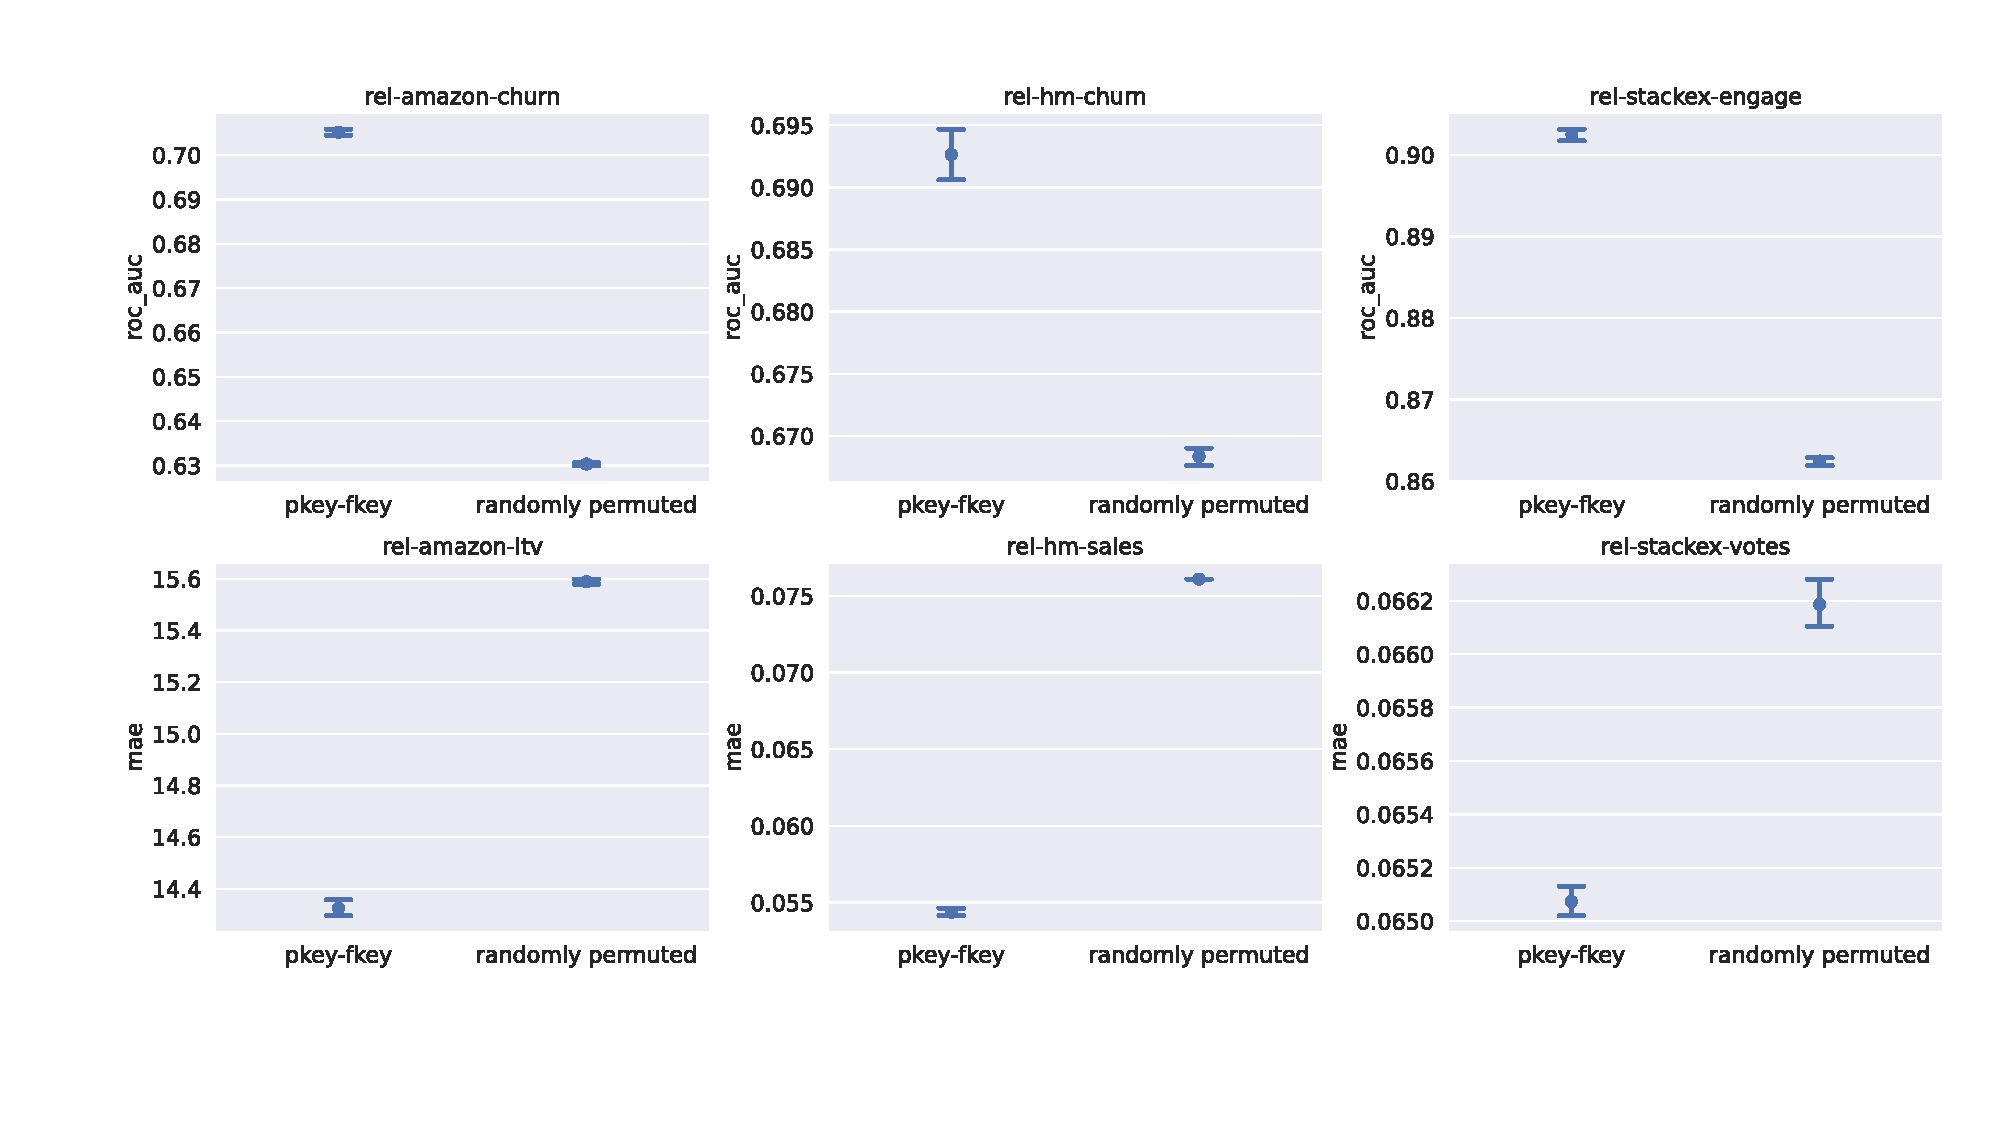
\includegraphics[width=1.\linewidth]{figs/crop_ablation_edge.pdf}
    \caption{Investigation on the role of leveraging primary-foreign key (pkey-fkey) edges for the GNN. At the top row are three node classification tasks with metric AUROC (higher is better) while at the bottom are three node regression tasks with metric MAE (lower is better), evaluated on the test set. We find that our proposal of using pkey-fkey edges for message passing is vital for GNN to achieve desirable performance on~\relbench. Error bars correspond to 95\% confidence interval.}
    \label{fig:ablation-edge}
\end{figure}

\textbf{Graph structure.} We first investigate the role of the graph structure we adopt for GNNs on~\relbench. Specifically, we compare the following two approaches of constructing the edges: \textbf{1.} \emph{Primary-foreign key (pkey-fkey)}, where the entities from two tables that share the same primary key and foreign key are connected through an edge; \textbf{2.} \emph{Randomly permuted}, where we apply a random permutation on the destination nodes in the primary-foreign key graph for each type of the edge while keeping the source nodes untouched. From Fig.~\ref{fig:ablation-edge} we observe that with random permutation on the primary-foreign key edges the performance of the GNN becomes much worse, verifying the critical role of carefully constructing the graph structure through, \eg, primary-foreign key as proposed in~\citet{fey2023relational}.

\begin{figure}[t!]
    \centering
    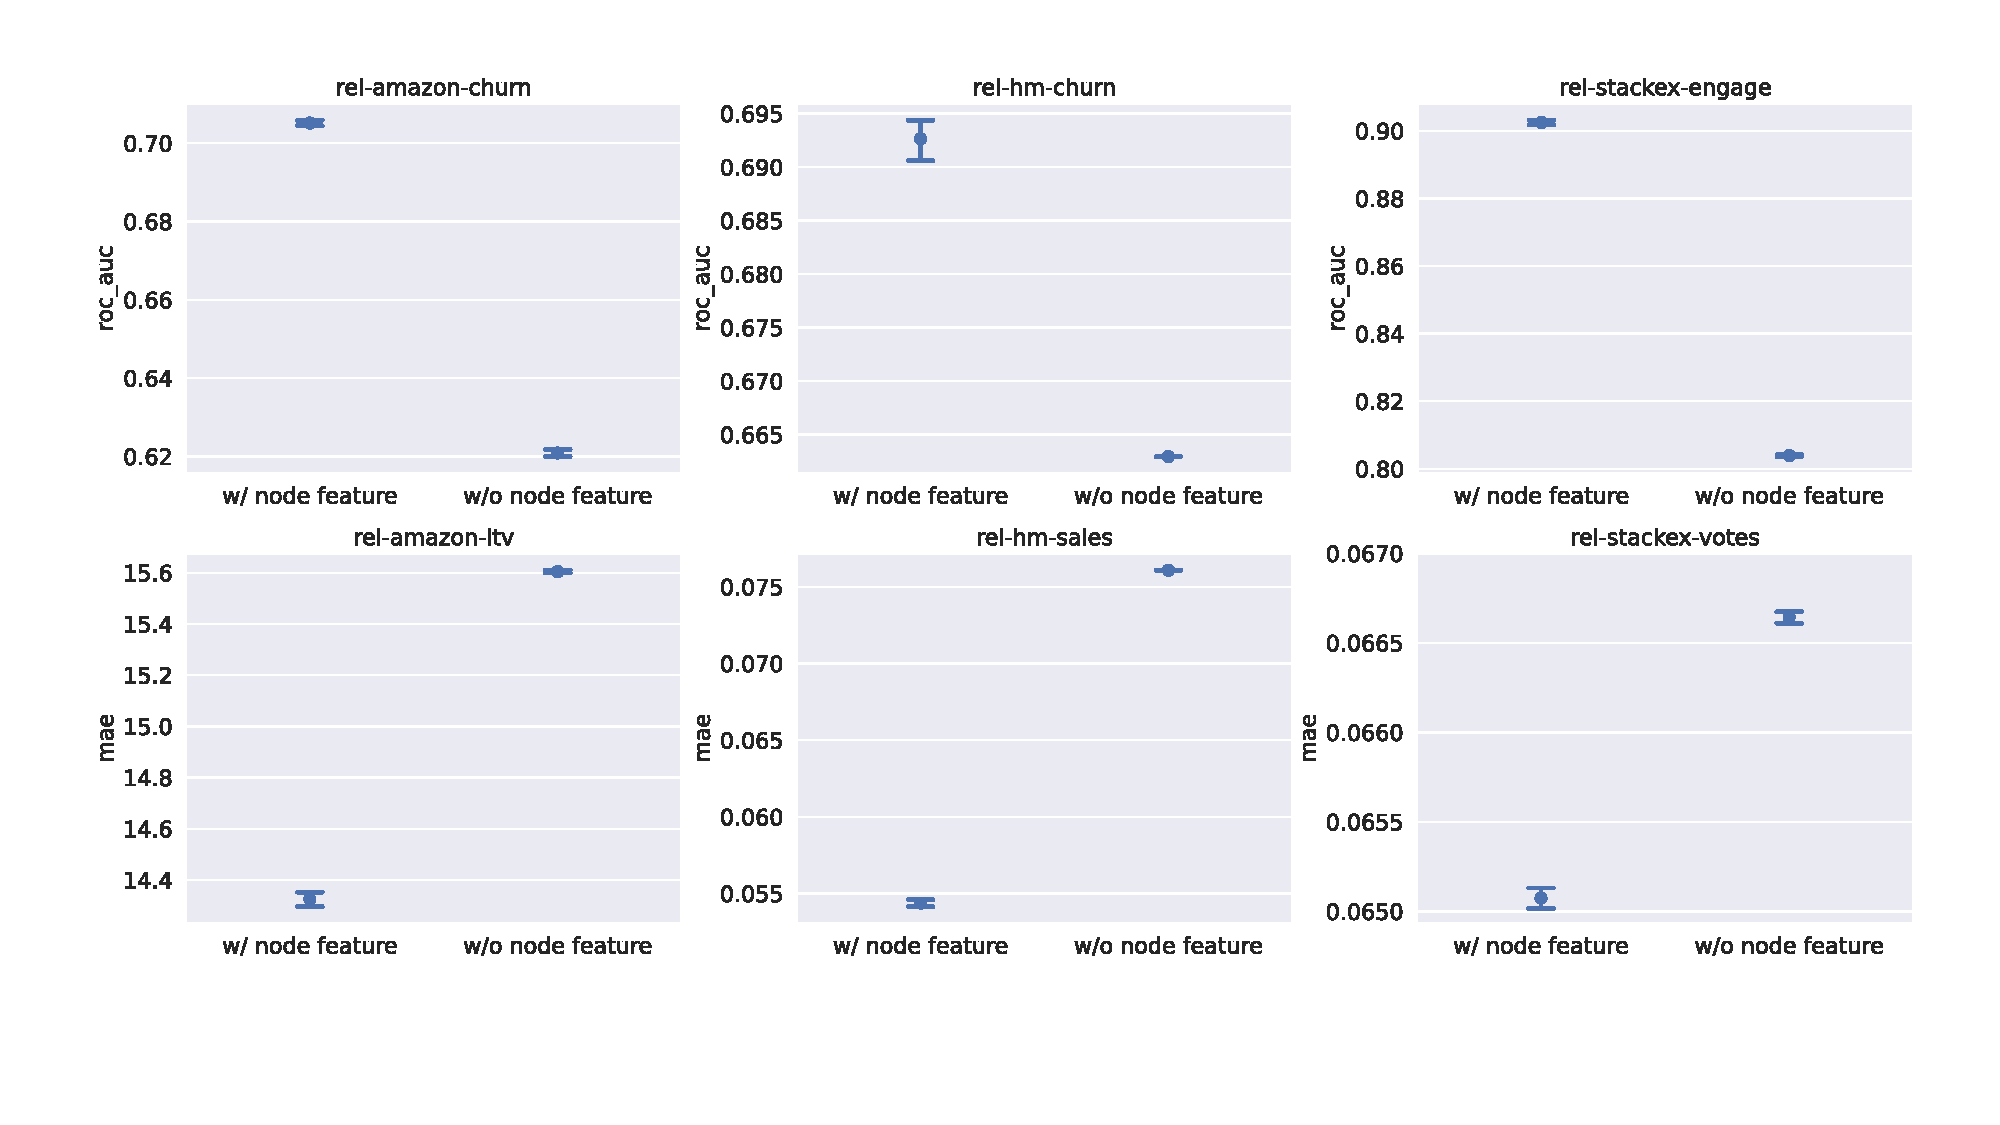
\includegraphics[width=1.\linewidth]{figs/crop_ablation_nodefeature.pdf}
    \caption{Investigation on the role of node features. At the top row are three node classification tasks with metric AUROC (higher is better) while at the bottom are three node regression tasks with metric MAE (lower is better), evaluated on the test set. We observe that leveraging node features is important for GNN. Error bars correspond to 95\% confidence interval.}
    \label{fig:ablation-nodefeature}
\end{figure}

\begin{figure}[t!]
    \centering
    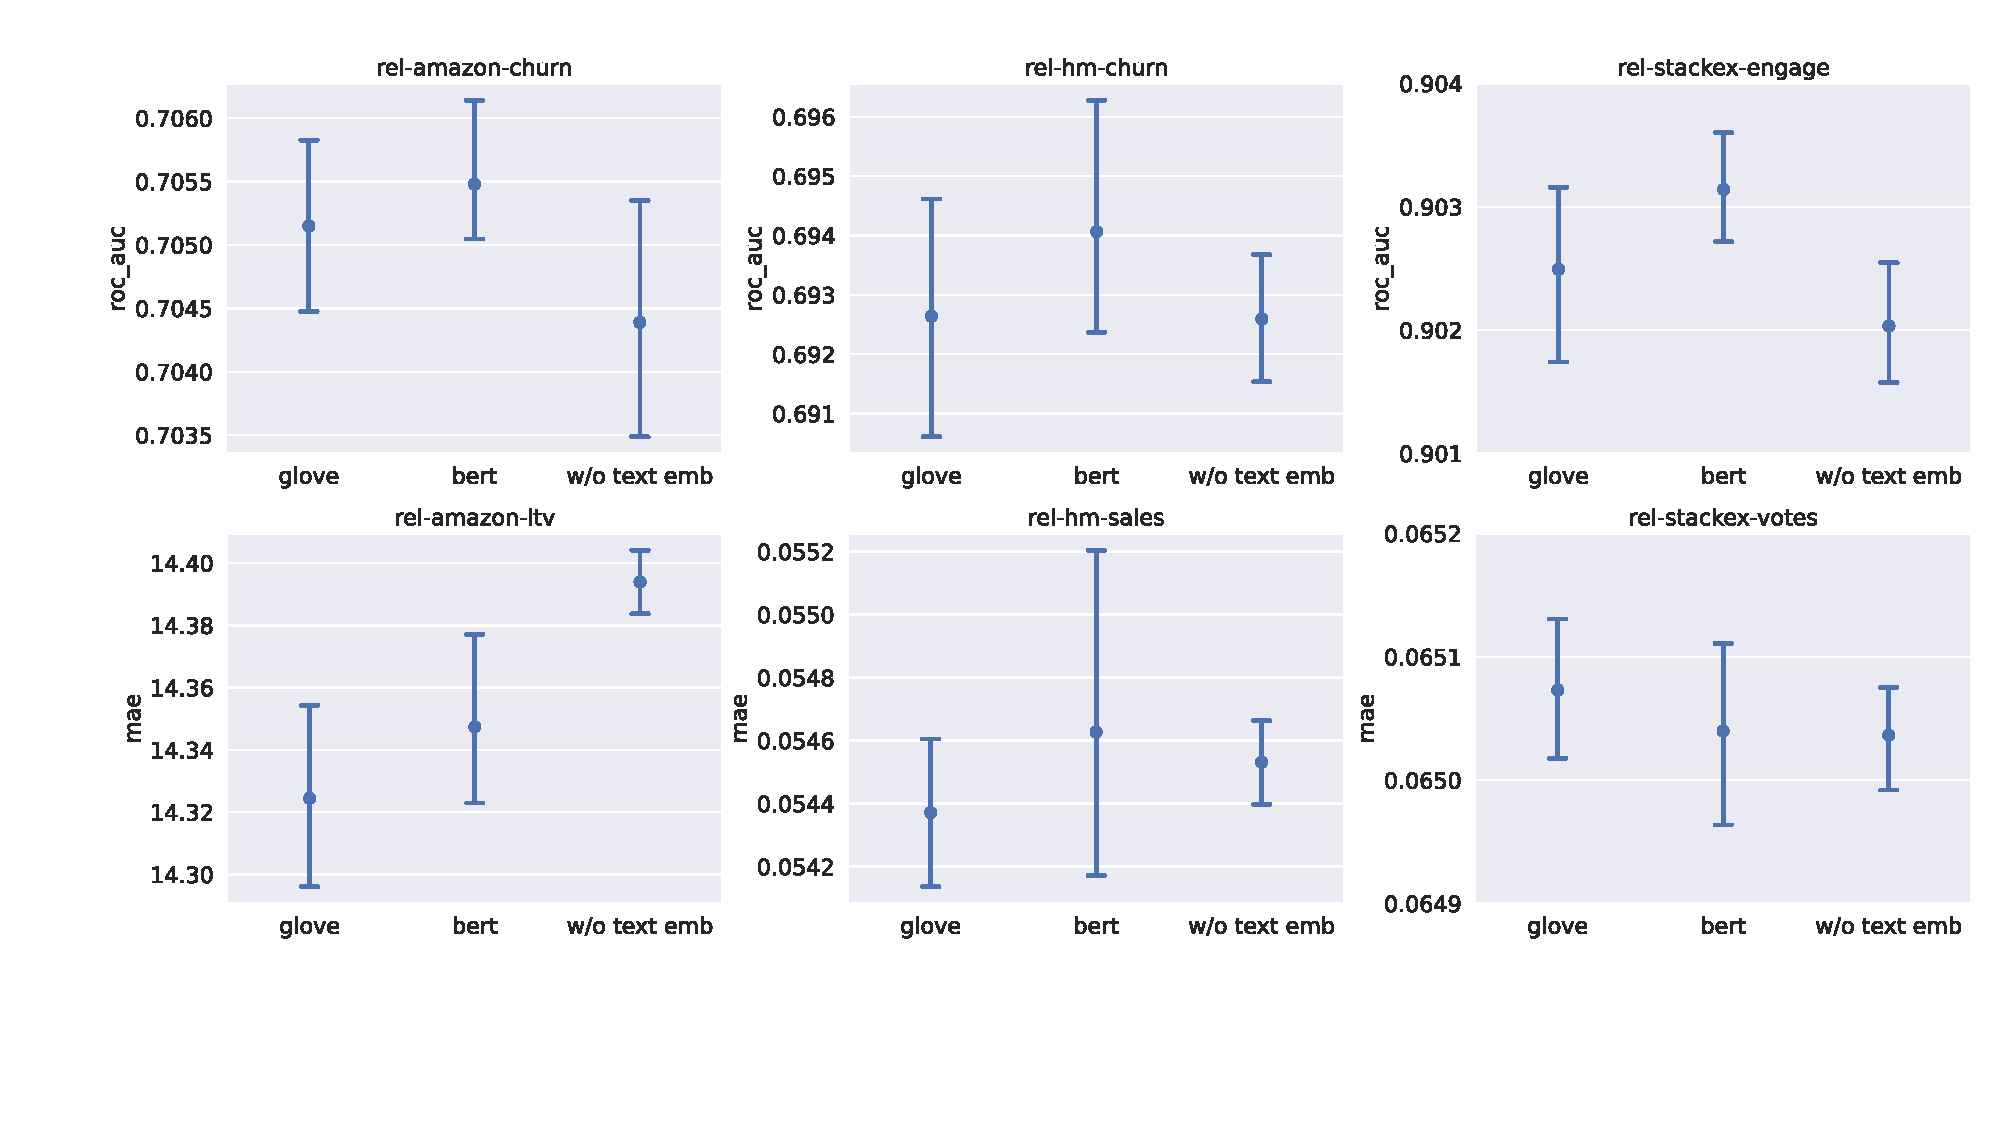
\includegraphics[width=1.\linewidth]{figs/crop_ablation_text.pdf}
    \caption{Investigation on the role of text embedding. At the top row are three node classification tasks with metric AUROC (higher is better) while at the bottom are three node regression tasks with metric MAE (lower is better), evaluated on the test set. We observe that adding text embedding using GloVe~\citep{pennington2014glove} or BERT~\citep{devlin2018bert} generally helps improve the performance. Error bars correspond to 95\% confidence interval.}
    \label{fig:ablation-textemb}
\end{figure}


\textbf{Node features and text embeddings.} Here we study the effect of node features used in~\relbench. In the experiments depicted in Fig.~\ref{fig:ablation-nodefeature}, we compare GNN (w/ node feature) with its variant where the node features are all masked by zeros (\ie, w/o node feature). We find that utilizing rich node features incorporated in our~\relbench dataset is crucial for GNN. Moreover, we also investigate, in particular, the approach to encode texts in the data that constitutes part of the node features. In Fig.~\ref{fig:ablation-textemb}, we compare GloVe text embedding~\citep{pennington2014glove} and BERT text embedding~\citep{devlin2018bert} with w/o text embedding, where the text embeddings are masked by zeros. We observe that encoding the rich texts in~\relbench with GloVe or BERT embedding consistently yields better performance compared with using no text features. We also find that BERT embedding is usually better than GloVe embedding especially for node classification tasks, which suggests that enhancing the quality of text embedding will potentially help achieve better performance.


\textbf{Temporal awareness.} We also investigate the importance of injecting temporal awareness into the GNN by ablating on the time embedding. To be specific, in the implementation we add a relative time embedding when deriving the node features using the relative time span between the timestamp of the entity and the querying seed time. Results are exhibited in Fig.~\ref{fig:ablation-timeemb}. We discover that adding the time embedding significantly enhance the performance across a diverse range of tasks, demonstrating the efficacy and importance of building up the temporal awareness into the model.

\begin{figure}[t!]
    \centering
    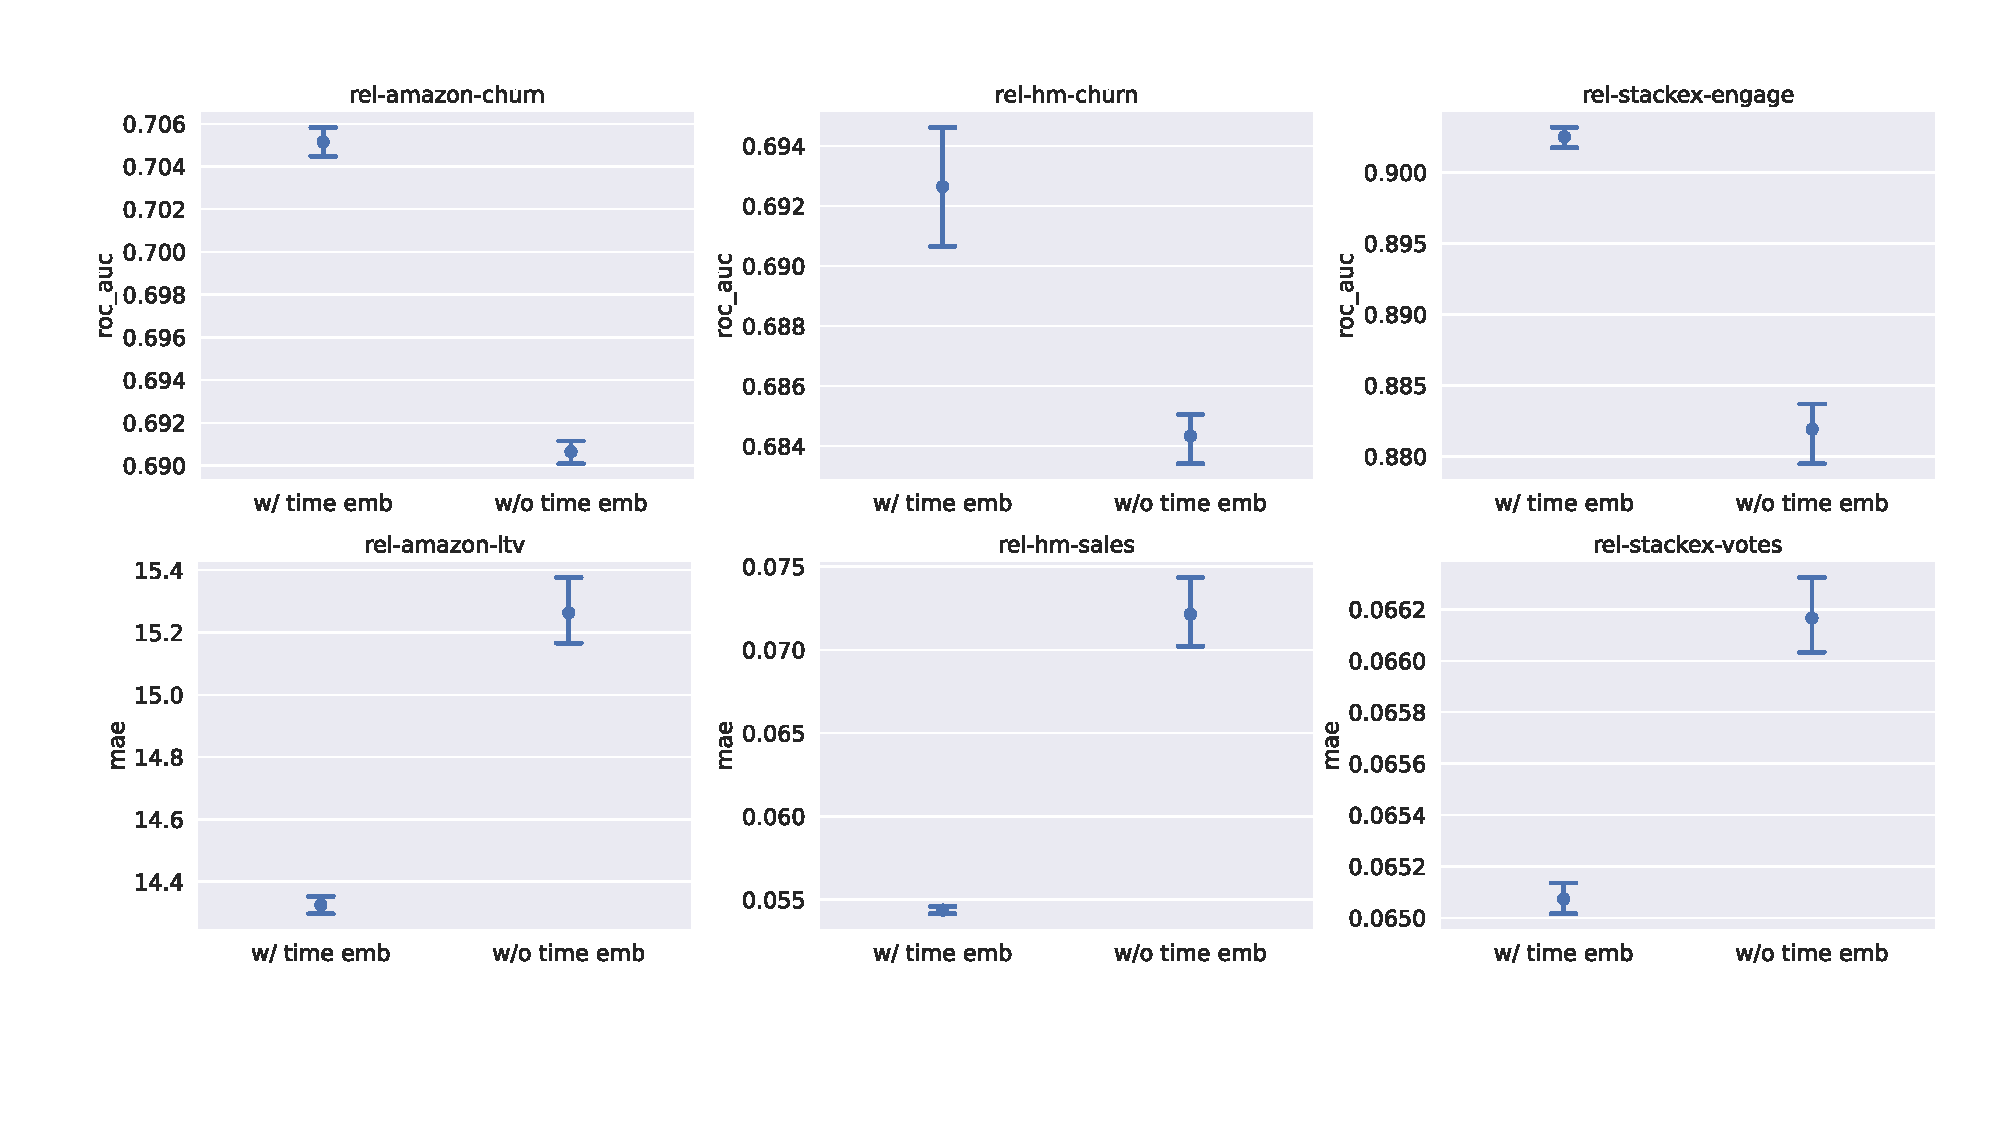
\includegraphics[width=1.\linewidth]{figs/crop_ablation_timeemb.pdf}
    \caption{Investigation on the role of time embedding. At the top row are three node classification tasks with metric AUROC (higher is better) while at the bottom are three node regression tasks with metric MAE (lower is better), evaluated on the test set. We find that adding time embedding to the GNN consistently boosts the performance. Error bars correspond to 95\% confidence interval.}
    \label{fig:ablation-timeemb}
\end{figure}


